% Created 2016-11-24 Thu 18:07
% Intended LaTeX compiler: xelatex
\documentclass[a4paper, titlepage]{article}
\usepackage{graphicx}
\usepackage{grffile}
\usepackage{longtable}
\usepackage{wrapfig}
\usepackage{rotating}
\usepackage[normalem]{ulem}
\usepackage{amsmath}
\usepackage{textcomp}
\usepackage{amssymb}
\usepackage{capt-of}
\usepackage{hyperref}
\usepackage[polish]{babel}
\usepackage{fontspec}
\defaultfontfeatures{Ligatures=TeX}
\setromanfont{Baskerville}
\setsansfont{Tahoma}[Scale=MatchLowercase]
\setmonofont{Hack}[Scale=MatchLowercase]
\author{Wojciech Polak, Klaudia Głocka, Rafał Ziembiński, Konrad Chojnecki}
\date{\today}
\title{Programowanie Zespołowe 2016\\\medskip
\large Bluetooth Messenger}
\hypersetup{
 pdfauthor={Wojciech Polak, Klaudia Głocka, Rafał Ziembiński, Konrad Chojnecki},
 pdftitle={Programowanie Zespołowe 2016},
 pdfkeywords={},
 pdfsubject={},
 pdfcreator={Emacs 25.1.1 (Org mode 9.0)}, 
 pdflang={Polish}}
\begin{document}

\maketitle
\tableofcontents

\clearpage
\section{Opis aplikacji}
\label{sec:orgd9d104d}
Aplikacja ma za zadanie połączenie dwóch lub więcej urządzeń, poprzez protokół komunikacyjny \emph{Bluetooth}, w celu zapewnienia podstawowej komunikacji w postaci wiadomości tekstowych.
\subsection{Użyte technologie}
\label{sec:orgd3acfa2}
Do stworzenia aplikacji użyto zestawu narzędzi firmy \emph{Xamarin}. Kod źródłowy aplikacji został napisany głównie w języku C\#.
Użyte biblioteki i oprogramowanie pozwoliło współdzielić kod dla wielu platform, tym samym umożliwiając szybki rozwój aplikacji zarówno na system \textbf{iOS} jak i \textbf{Android}.
\subsection{Zarys architektury aplikacji}
\label{sec:org014a08f}
Aplikacja została stworzona w oparciu o wzorzec projektowy \emph{Model - View - Controller}.

\begin{center}
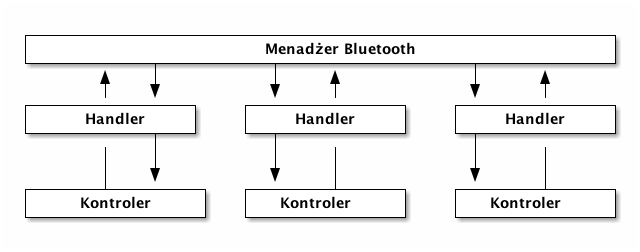
\includegraphics[width=.9\linewidth]{zarys.png}
\end{center}

\subsubsection{Moduł Menadżera Bluetooth}
\label{sec:orgab0d942}
Menadżer Bluetooth odpowiada za najniższą warstwę aplikacji. Każdy z systemów - odpowiednio \textbf{iOS} jak i \textbf{Android} posiadają inne Programistyczne Interfejsy Aplikacji (w skrócie \emph{API}). Najniższa warstwa będąca \emph{najbliżej sprzętu} została rozdzielona pomiędzy systemy. Dlatego ten menadżer został zaimplementowany jako dwa moduły.

Ponieważ wymagane jest aby aplikacja w przyszłości była łatwo rozszerzalna, została wprowadzona warstwa abstrakcji - \texttt{IBluetoothManager} która służy jako punkt wyjścia i wejścia dla innych modułów.

\begin{center}
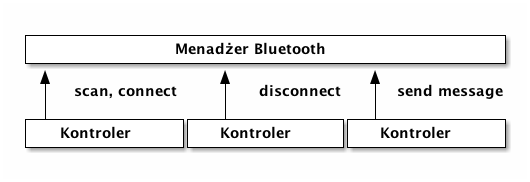
\includegraphics[width=.9\linewidth]{BM.png}
\end{center}

\subsubsection{Asynchroniczność aplikacji}
\label{sec:org43b797d}
Aplikacja jest zależna od zasobów zewnętrznych takich jak sieć \emph{Bluetooth}. W momencie gdy system czeka na nawiązanie połączenia z drugą komórką jest wymagane aby użytkownik cały czas miał aplikację interaktywną i responsywną. 

Aby aplikacja nie blokowała interfejsu użytkownika wszystkie akcje wykonywane przez warstwy niższe i pośrednie muszą być \textbf{asynchroniczne}.
Rozwiązaniem są moduły \texttt{Handlera} których zadaniem jest reakcja na wydarzenia.
\subsubsection{Moduł \texttt{Handler}}
\label{sec:orgc7b1413}
W momencie gdy zadanie zostanie wykonane (np. użytkownik zostanie połączony z innym), wiadomość zostaje wysłana do odpowiedniego \texttt{Handler} który reaguje w odpowiedni sposób do danych wejściowych.

\begin{center}
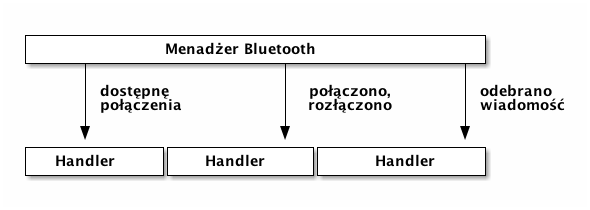
\includegraphics[width=.9\linewidth]{Handler.png}
\end{center}

W projekcie znajdują się dwa moduły typu \texttt{Handler}
\begin{enumerate}
\item Moduł \texttt{Message Handler}
\texttt{Message Handler} odpowiada za łączenie z innymi użytkownikami.
Do zadań tego modułu należą:
\begin{itemize}
\item Reakcja na pobraną listę dostępnych w pobliżu użytkowników - pseudonimy użytkowników są wyświetlane na ekranie.
\item Reakcja na połączenie się z danym użytkownikiem - następuje zmiana widoku na widok wysłanych i odebranych wiadomości.
\end{itemize}
\item Moduł \texttt{Connection Handler}
\texttt{Connection Handler} odpowiada za reakcję na wiadomości odebrane od innego użytkownika. Wiadomości takie są wyświetlane w czytelnej formie na ekranie telefonu.
\end{enumerate}
\subsubsection{Modele}
\label{sec:orgc0d330a}

\begin{center}
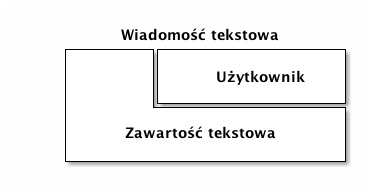
\includegraphics[width=.9\linewidth]{models.png}
\end{center}

\begin{enumerate}
\item Użytkownik
\label{sec:org5dd4790}
Aplikacja przechowuje informacje o użytkowniku takie jak:
\begin{itemize}
\item pseudonim
\item unikalny identyfikator oparty o technologię \texttt{GUID4}
\end{itemize}
\item Wiadomość
\label{sec:org74946ed}
Wysyłane i odbierane wiadomości mają format:
\begin{itemize}
\item Użytkownik
\item Wiadomość tekstowa
\end{itemize}
\end{enumerate}
\subsubsection{Kontrolery}
\label{sec:orgdfd7432}
Kontrolery odpowiadają za zarządzanie danymi które zostały odebrane przez moduły \texttt{Handler}.
Często wymagane jest aby dane te zostały odpowiednio spreparowane zanim zostaną wyświetlone na ekranie.
Dobrą praktyką jest, aby w dalszych widokach \textbf{nie było żadnej logiki biznesowej}. Dlatego każda operacja na danych musi się odbyć w kontrolerze.

Kontrolery są modułami które odbierają wydarzenia (np. naciśnięcie przycisku, wpisanie tekstu, gesty czy ruch zarejestrowany przez akcelerator) które zostały wykonane w odpowiednich widokach.
Kontrolery reagują wydarzenia i na podstawie zawartości wydarzeń przesyłają odpowiednie komendy do pozostałych modułów, najczęściej do Menadżera Bluetooth.
\subsubsection{Widoki}
\label{sec:orgc26f2e5}
Aplikacja składa się z dwóch widoków.
\begin{enumerate}
\item Widok z możliwymi połączeniami. 
W tym widoku użytkownik może zobaczyć wszystkich innych użytkowników, którzy są w zasięgu.
Urządzenie skanuje obszar w określonym interwale czasowym.
Użytkownik może nawiązać bezpośrednie połączenie z jednym użytkownikiem tym samym przechodzą do widoku drugiego.
\item Widok wymiany wiadomości.
W tym widoku użytkownik wysyła i odbiera wiadomości nadane przez drugiego użytkownika. Na raz możliwa jest rozmowa tylko z jednym użytkownikiem.
Użytkownik oprócz wysyłania wiadomości może także zakończyć rozmowę tym samym wracając do widoku pierwszego.
\end{enumerate}
\section{Podział prac}
\label{sec:org0da3699}
\subsection{Rafał Ziembiński - moduł \texttt{BluetoothManager} dla systemu Android}
\label{sec:org561f1e1}
\subsection{Klaudia Głocka - moduł \texttt{ConnectionHandler}}
\label{sec:org0502abe}
\subsection{Konrad Chojnecki - moduł \texttt{MessageHandler}}
\label{sec:org6085e76}
\subsection{Wojciech Polak - moduł \texttt{BluetoothManager} dla systemu iOS}
\label{sec:org9716bc0}
\section{Stan prac}
\label{sec:org370be41}
\subsection{Na dzień 01-11-2016}
\label{sec:org8ff9b79}
\begin{enumerate}
\item Przerwa w pracy w wyniku dni wolnych od pracy
\item Poprawa dokumentu opisującego projekt. Wykorzystanie w tym celu \LaTeX{}.
\item Konfiguracja środowisk programistycznych:
\begin{itemize}
\item Próby instalacji IDE, wymaganych bibliotek i narzędzi pracy
\item Konfiguracja maszyn wirtualnych oraz urządzeń natywnych
\end{itemize}
\end{enumerate}
\subsection{Na dzień 10-11-2016}
\label{sec:org124e069}
\begin{enumerate}
\item Reinstalacja systemu operacyjnego Microsoft Windows na jednym stanowisku pracy, konfiguracja wszystkich potrzebnych bibliotek, narzędzi i edytorów.
\item Usunięcie Visual Studio 2013 na drugim stanowisku pracy. Konfiguracja Visual Studio 2015.
\item Aktualizacja dokumentacji o grafy i wykresy połączeń pomiędzy modułami
\end{enumerate}
\subsection{Na dzień 17-11-2016}
\label{sec:org3798f77}
\begin{itemize}
\item \textbf{Rafał Ziembiński}:
Reinstalacja całego systemu operacyjnego umożliwiła uruchomienie emulatora Android wraz z działającym prototypem aplikacji.
\begin{center}
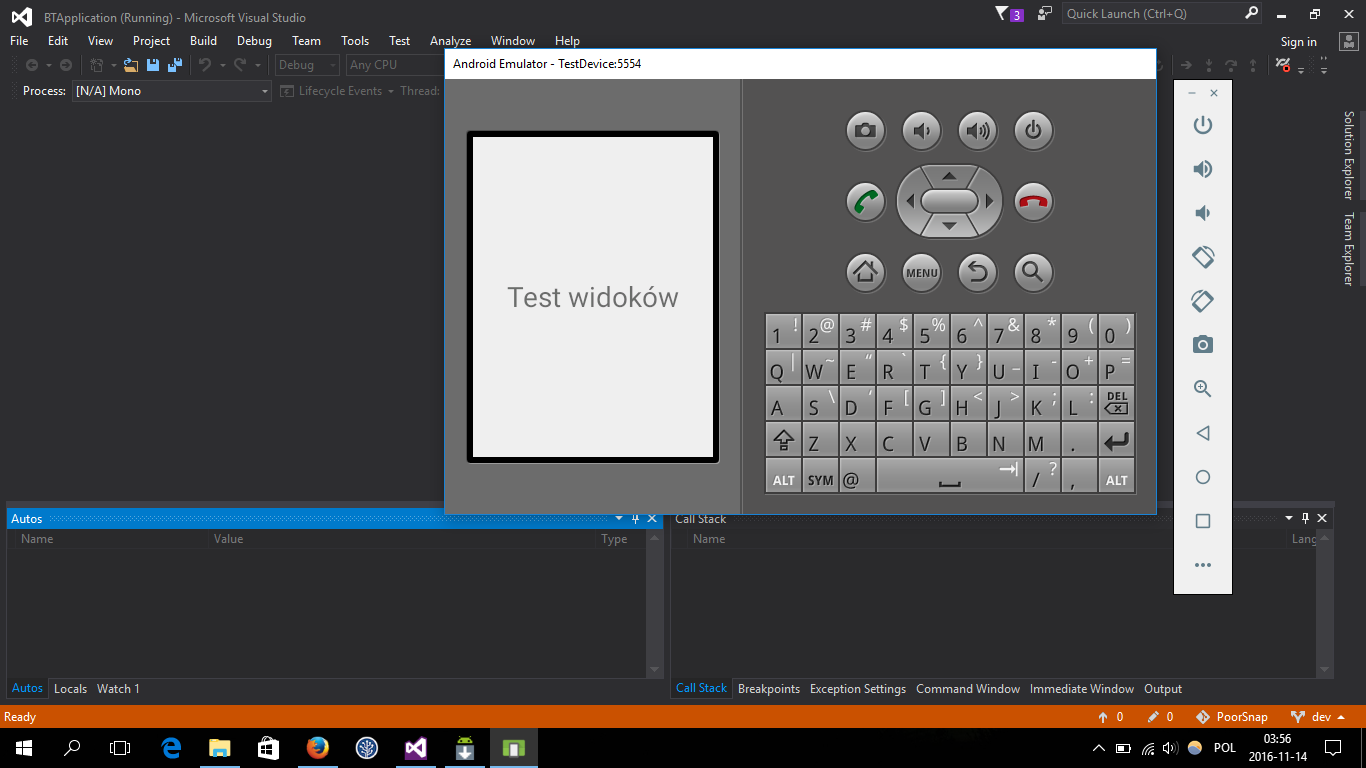
\includegraphics[width=.9\linewidth]{./emulator.png}
\end{center}
Rozpoczęty research w sprawie Bluetooth na Android.
\item \textbf{Klaudia Głocka}:
Rozpoczęty research i pierwsze testy związane z obsługą Visual Studio.
Rozpoczęty kurs języka C\#.
Pierwsze próby z systemem kontroli wersji Git.
\item \textbf{Konrad Chojnecki}:
Research dotyczący architektury zestawu narzędzi Xamarin.
Research dotyczący widoków aplikacji.
\item \textbf{Wojciech Polak}:
Dalszy research w sprawie Bluetooth na iOS:
Głównie oparty o \url{https://developer.xamarin.com/api/namespace/CoreBluetooth/}
API \texttt{CoreBluetooth} pozwala na pracę z \texttt{Bluetooth Low Energy}.
Wciąż nie jest pewne, czy będzie możliwa bezproblemowa komunikacja między iOS a Android.
Znalezione zostało rozwiązanie pośrednie - gotowy moduł działający zarówno dla iOS jak i dla Android - \url{https://components.xamarin.com/view/ch.arendi.blelibrary}
\end{itemize}
\subsection{Na dzień 24-11-2016}
\label{sec:org1f7d600}
\begin{itemize}
\item \textbf{Rafał Ziembiński}
Pobieranie emulatorów różnych urządzeń Android w celu sprawdzenia integralności aplikacji na różnych platformach i wersjach systemu.
Badanie przestrzeni nazw \texttt{Android.Bluetooth}. Sprawdzenie modułu działającego zarówno na iOS jak i dla Android.
\item \textbf{Klauda Głocka}
Przygotowanie widoków aplikacji oraz zdobywanie wiedzy jak je podpiąć pod moduł \texttt{MessageHandler}.
\item \textbf{Wojciech Polak}
Znalezione \texttt{API} \texttt{ExternalAccessory} pozwalające urządzeniom iOS na interakcje z urządzeniami Bluetooth.
[\url{https://developer.xamarin.com/api/namespace/ExternalAccessory/}]
Aktualizacja środowiska Xamarin Studio z powodów wymuszonej aktualizacji \texttt{IDE} XCode 8.
Walka z błędami przy wdrażaniu na natywne urządzenie.
\end{itemize}
\end{document}
